	The following python code computes the length of the altitude $\vec{AD}$ in Fig.\ref{fig:1.2.5_qtwo}.
	\begin{lstlisting}
	./solutions/5/codes/triangle/q2.py
	\end{lstlisting}
	
	\begin{figure}[!ht]
	\centering
	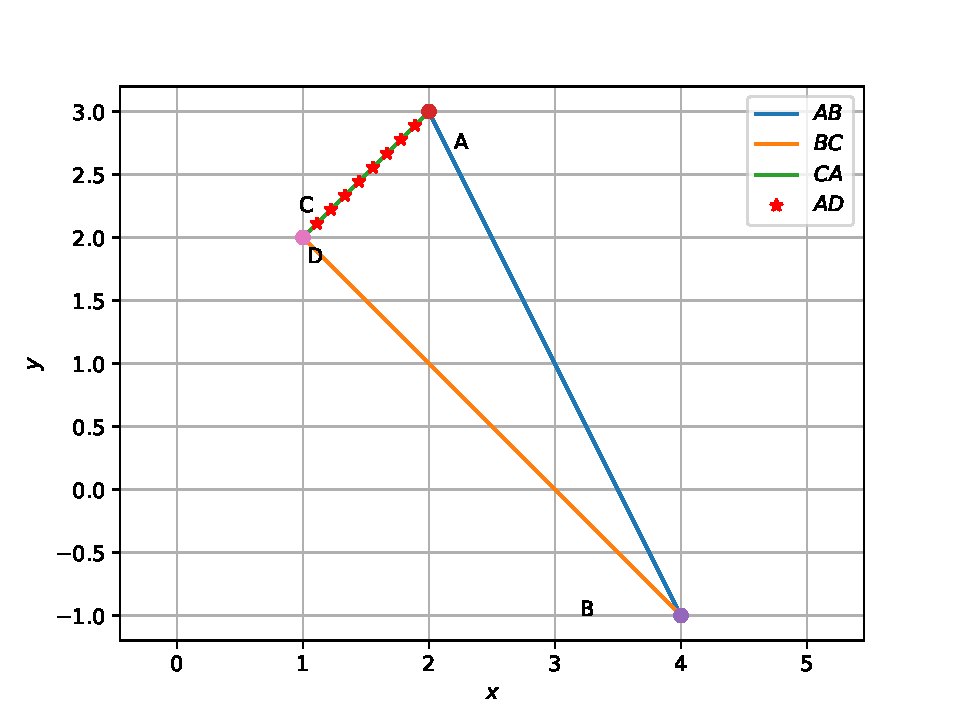
\includegraphics[width=\columnwidth]{./solutions/5/figs/triangle/q2.eps}
	\caption{Triangle of Q.1.2.5}
	\label{fig:1.2.5_qtwo}	
	\end{figure}
	
In $\triangle ABC$, 
	\begin{align}
\brak{\vec{A}-\vec{C}}^T\brak{\vec{B}-\vec{C}} = 0
	\end{align}
Hence, $ABC$ is a right triangle. The direction vector of $BC$ is 
\begin{align}
\brak{\vec{B}-\vec{C}} = \myvec{3\\-3}
\end{align}
Hence, the equation of $AD$ is 
\begin{align}
\brak{\vec{B}-\vec{C}}^T \brak{\vec{x}-\vec{A}} &= 0
\\
\implies 		\myvec{1&-1}\vec{x} &= -1
\end{align}
The length of the altitude is obtained as $\norm{\vec{A-D}} = 1.414$
	
	
	
	
